%###########################PRESENTACION##########################################
%Modo presentación
\documentclass[14pt]{beamer}

%Modo handout
%\documentclass[handout,compress]{beamer}
%\usepackage{pgfpages}
%\pgfpagesuselayout{4 on 1}[border shrink=1mm]

\usepackage{graphicx,pstricks}
\usepackage{beamerthemeCambridgeUS}
\usepackage{subfig}
\usepackage{tikz}
\usepackage{amsmath}
\usepackage{hyperref}

\graphicspath{{G:/My Drive/FIGURAS/}}
\setbeamercovered{transparent}

\title[DEM]{ANÁLISIS GEOESPACIAL}
\author[Edier Aristizábal]{Edier V. Aristizábal G.}
\institute{\emph{evaristizabalg@unal.edu.co}}
\date{\tiny{(Versión:\today)}}
\usepackage{textpos}

\addtobeamertemplate{headline}{}{%
	\begin{textblock*}{2mm}(.9\textwidth,0cm)
	\hfill
\includegraphics[height=1cm]{un}
	\end{textblock*}
			}
%############################INICIO#############################################
\begin{document}
\begin{frame}
\titlepage
\centering
	
\includegraphics[width=5cm]{unal}\hspace*{4.75cm}~%
   	
\includegraphics[width=2cm]{logo3}
\end{frame}
%################################SLIDE
\begin{frame}
\begin{figure}[]
 \centering
  \begin{picture}(10,10)  
    \put(-170,-110){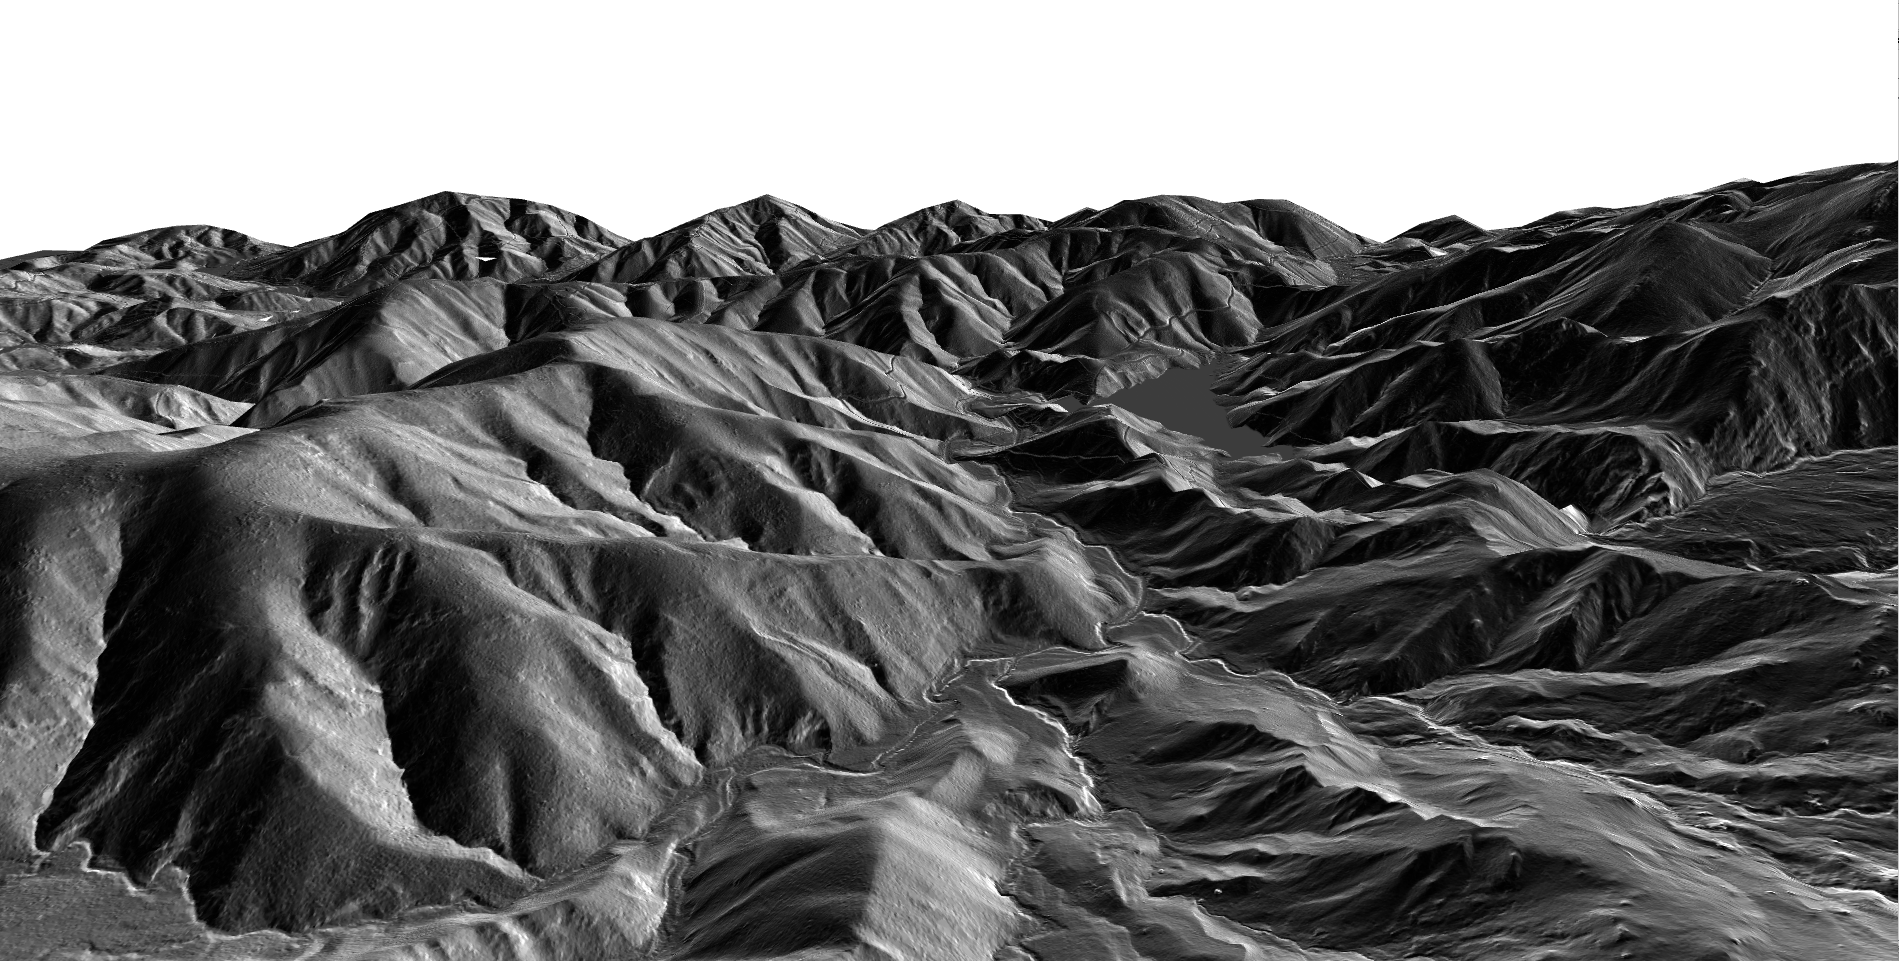
\includegraphics[scale=0.18]{dsm2}}
    \put(-140,60){\color{black}{\huge Digital Elevation Models}}
    \put(-170,-127) {\tiny{https://medium.com/on-location/from-points-to-pixels-creating-digital-elevation-models-from-open-topography-point-clouds}}
    \end{picture}
\end{figure}
\end{frame}
%################################SLIDE
\begin{frame}
\frametitle{DEM}
%\framesubtitle{}
\begin{columns}
		\begin{column}{.30\linewidth}
		 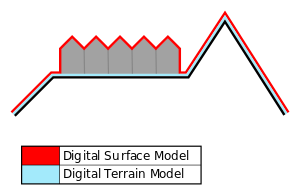
\includegraphics[width=4cm]{dtm3}
		\end{column}
		\begin{column}{.70\linewidth}
			 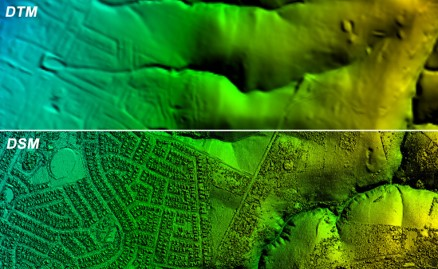
\includegraphics[width=8cm]{dtm2}
		\end{column}
	\end{columns}
\end{frame}
%################################SLIDE
\begin{frame}
\frametitle{DEM}
  \begin{figure}
    \centering
    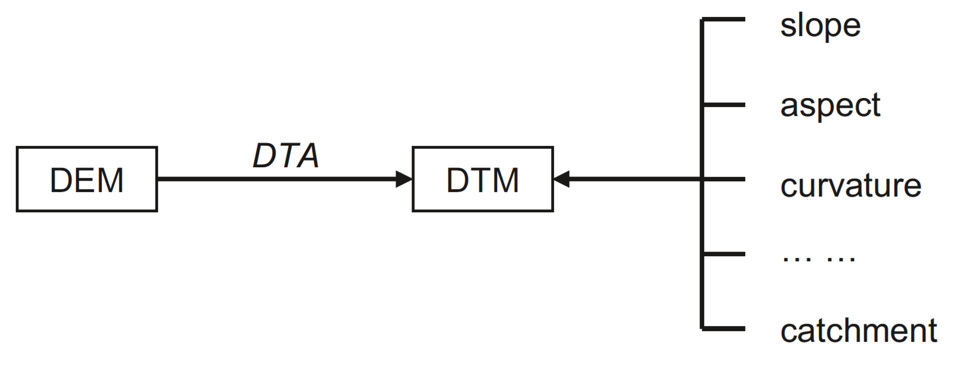
\includegraphics[height=.5\textheight]{dtm}
    %\caption{This is the caption.}
  \end{figure}
\end{frame}
%################################SLIDE
\begin{frame}
\frametitle{Modelos Digitales de Elevación (DEM)}
  \begin{figure}
    \centering
    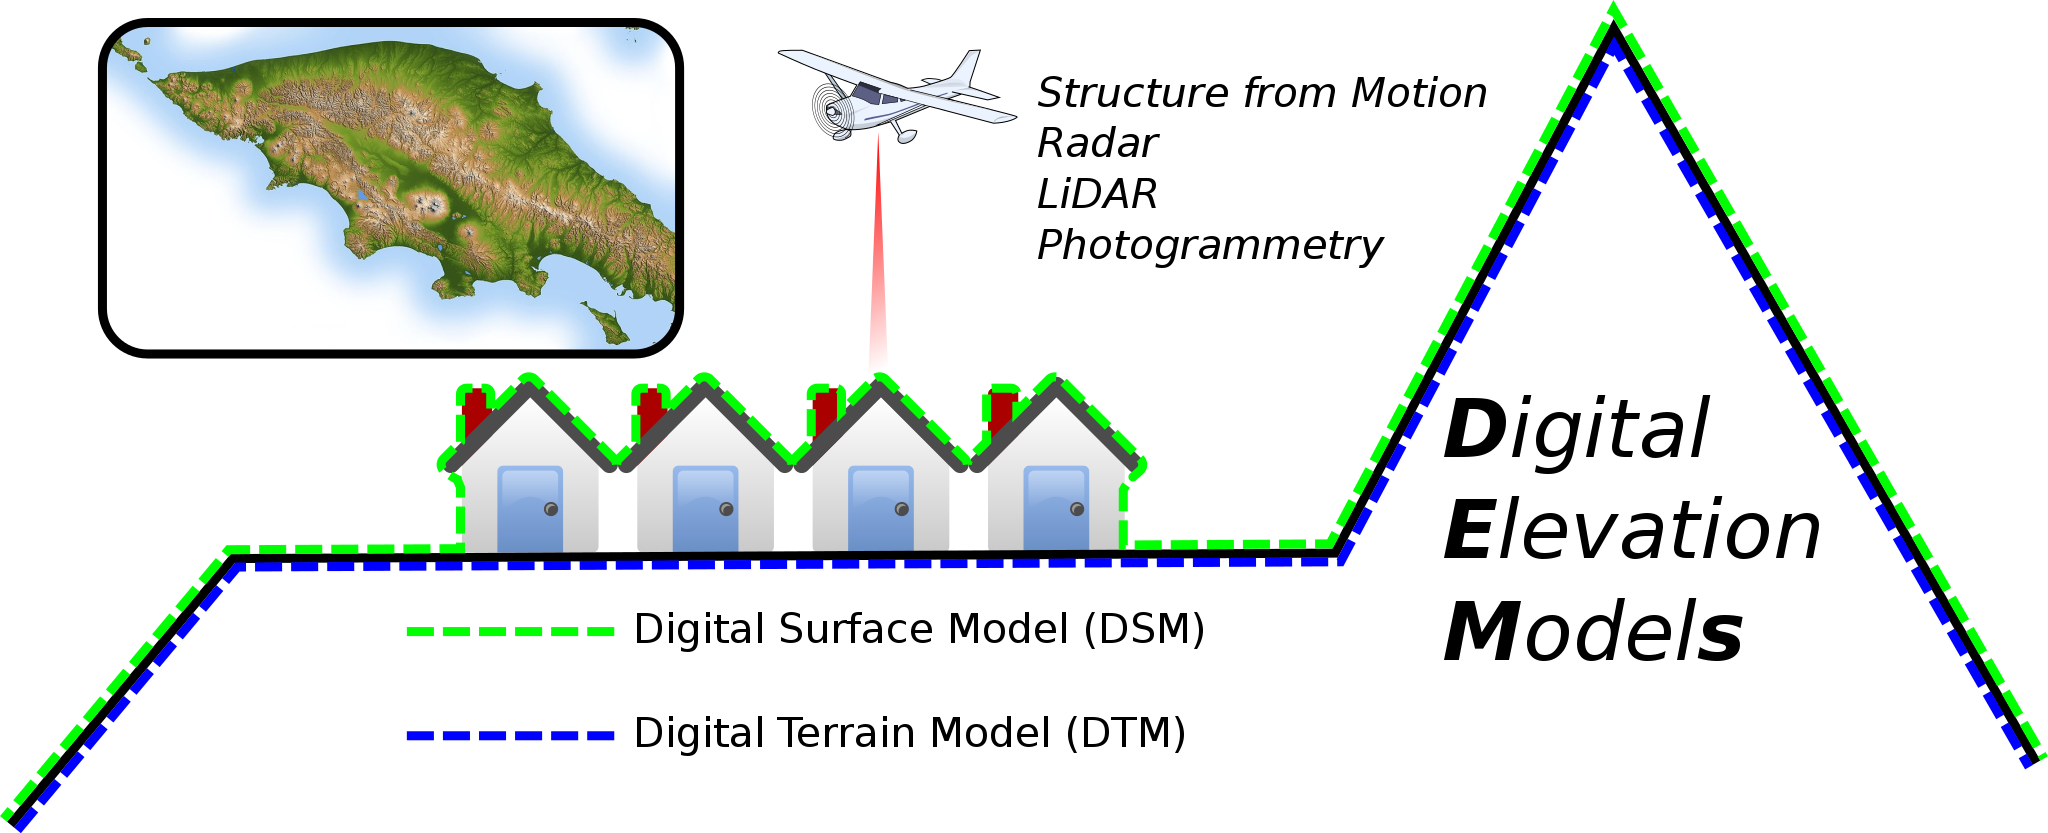
\includegraphics[height=.5\textheight]{dsm}\vfill
\tiny{Arbeck / CC BY (https://creativecommons.org/licenses/by/4.0)}
  \end{figure}
\end{frame}
%################################SLIDE
\begin{frame}
\frametitle{DTM}
%\framesubtitle{}
  \begin{figure}
    \centering
    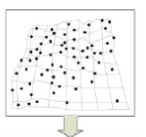
\includegraphics[width=2cm]{dem3}
    %\caption{This is the caption.}
   \end{figure}
\begin{columns}
		\begin{column}{.5\linewidth}
		 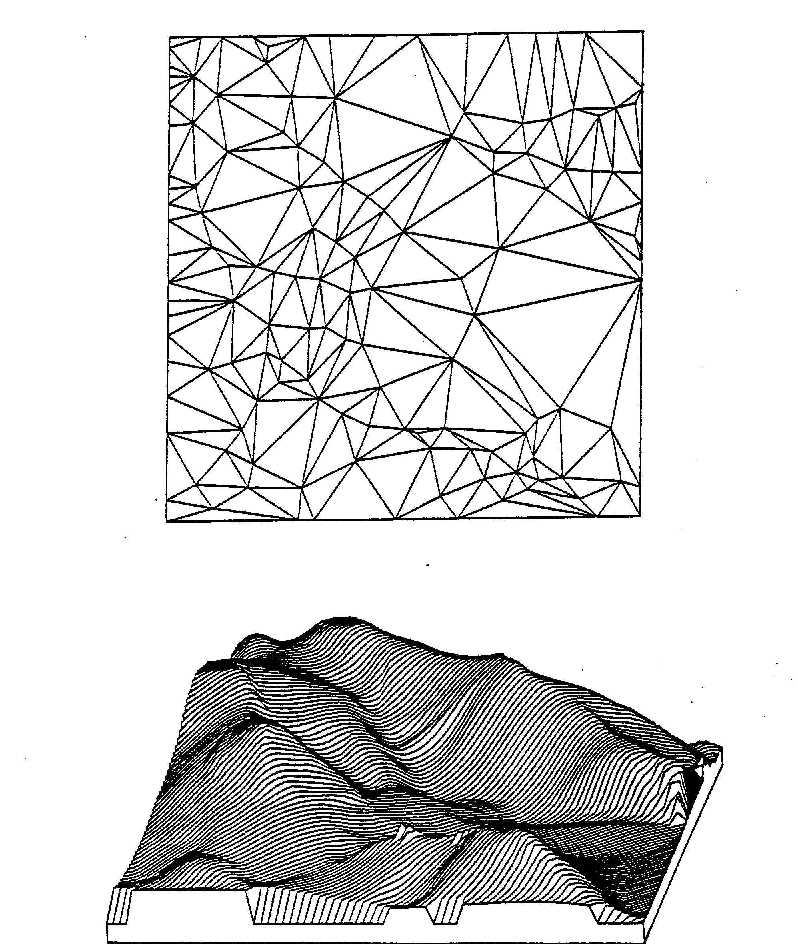
\includegraphics[width=4cm]{tin}
		\end{column}
		\begin{column}{.5\linewidth}
			 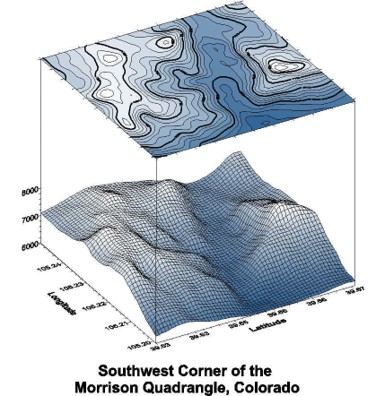
\includegraphics[width=4cm]{rast1}
		\end{column}
\end{columns}
\end{frame}
%################################SLIDE
\begin{frame}
  \begin{figure}
    \centering
    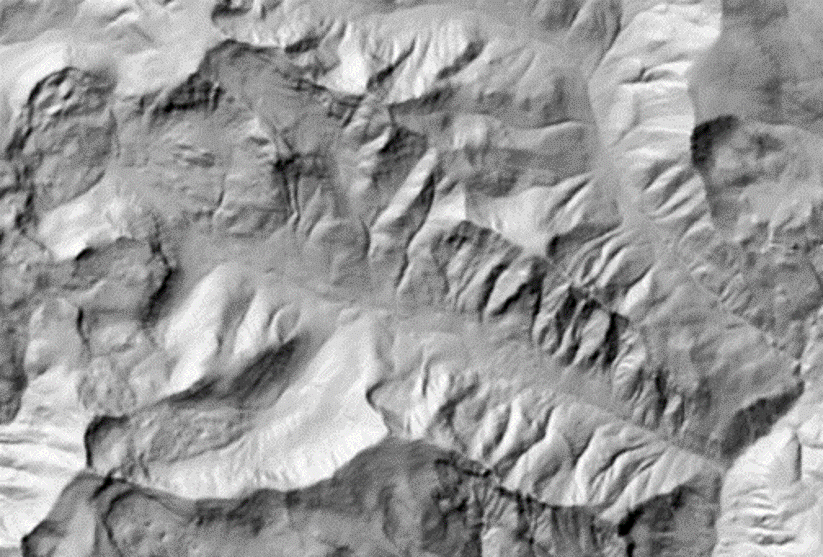
\includegraphics[height=.8\textheight]{dtm5}
    %\caption{This is the caption.}
  \end{figure}
\end{frame}
%################################SLIDE
\begin{frame}
  \begin{figure}
    \centering
    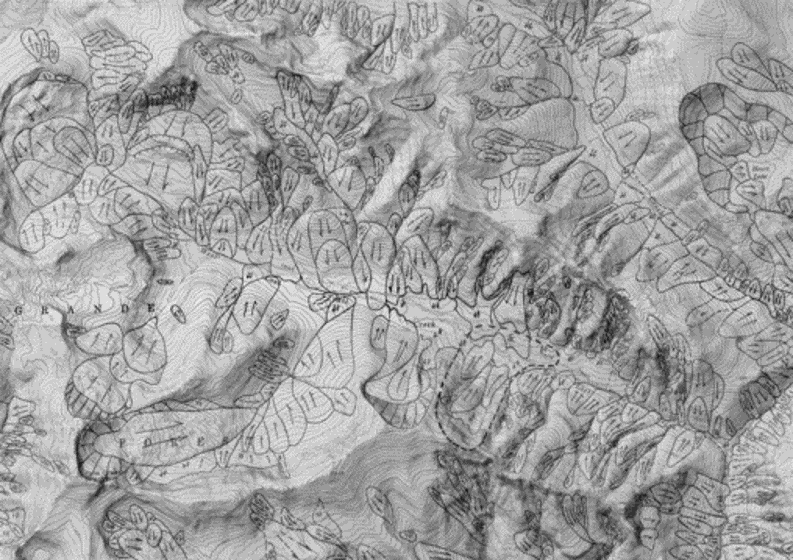
\includegraphics[height=.8\textheight]{dtm6}
    %\caption{This is the caption.}
  \end{figure}
\end{frame}
%################################SLIDE
\begin{frame}
\frametitle{Geomorfometría}
  \begin{figure}
    \centering
    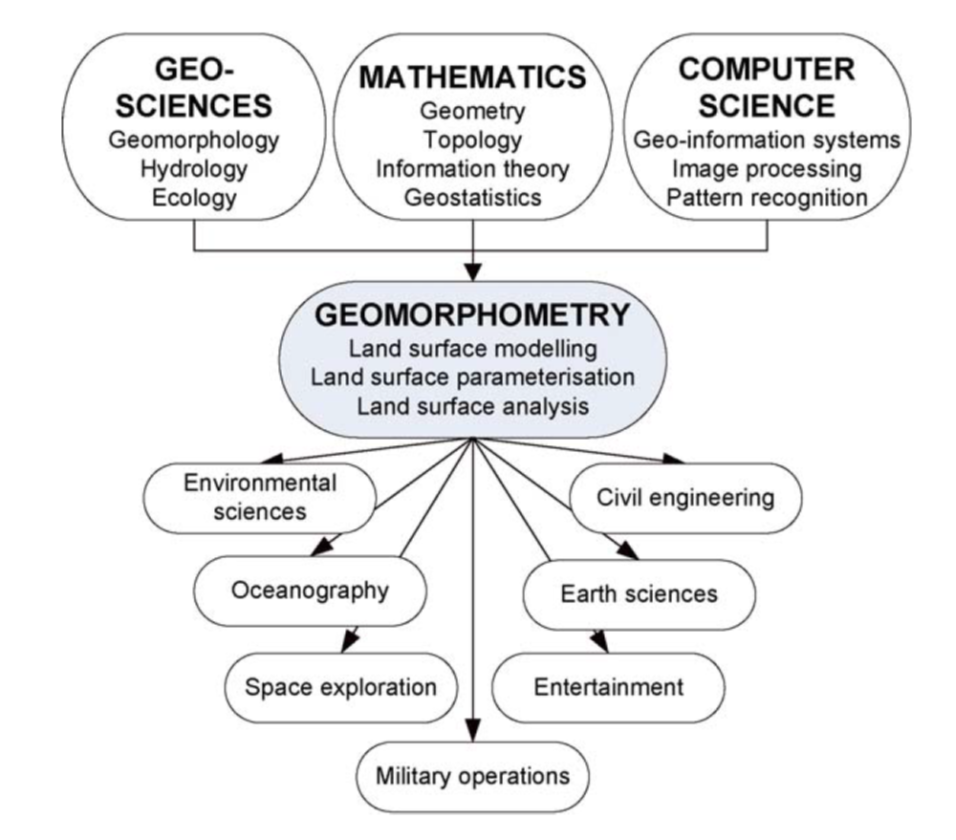
\includegraphics[height=.7\textheight]{geomorfometria}
    %\caption{This is the caption.}
  \end{figure}
\end{frame}
%################################SLIDE
\begin{frame}
  \begin{figure}
    \centering
    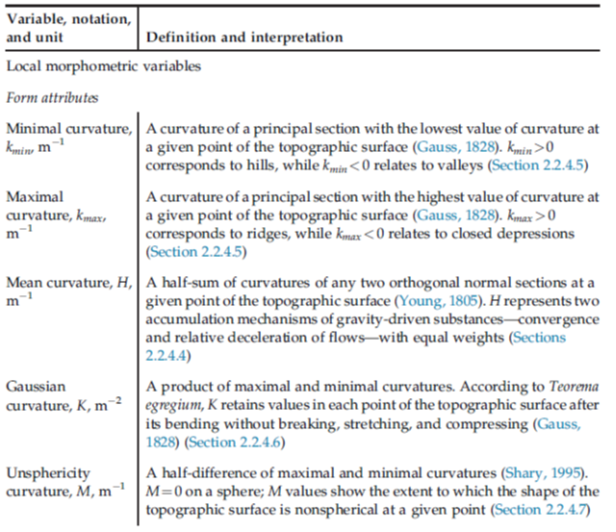
\includegraphics[height=.8\textheight]{indices}
    %\caption{This is the caption.}
  \end{figure}
\end{frame}
%################################SLIDE
\begin{frame}
  \begin{figure}
    \centering
    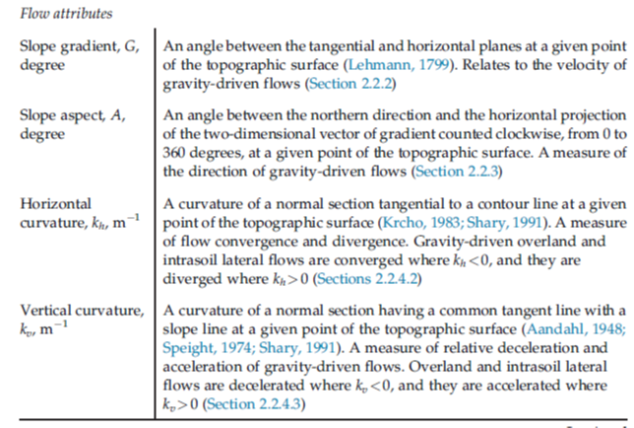
\includegraphics[height=.8\textheight]{indice1}
    %\caption{This is the caption.}
  \end{figure}
\end{frame}
%################################SLIDE
\begin{frame}
  \begin{figure}
    \centering
    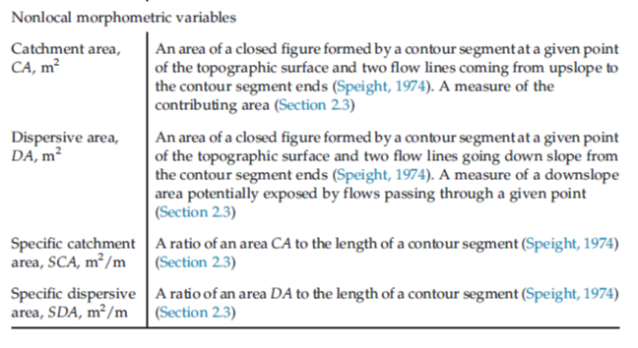
\includegraphics[height=.7\textheight]{indice3}
    %\caption{This is the caption.}
  \end{figure}
\end{frame}
%################################SLIDE
\begin{frame}
  \begin{figure}
    \centering
    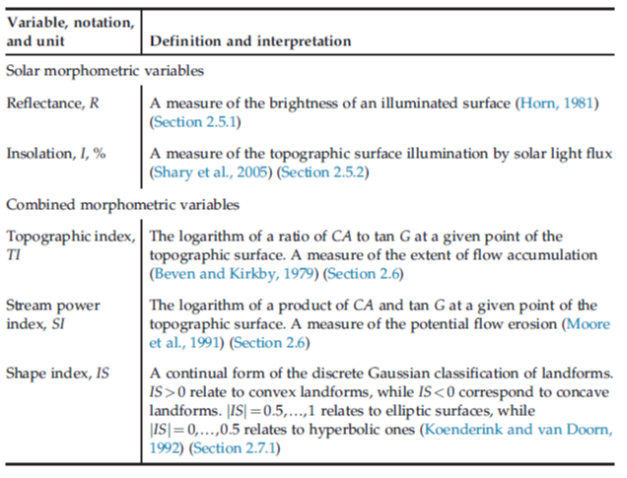
\includegraphics[height=.9\textheight]{indice4}
    %\caption{This is the caption.}
  \end{figure}
\end{frame}
%################################SLIDE
\begin{frame}
\frametitle{Pendiente}
  \begin{figure}
    \centering
    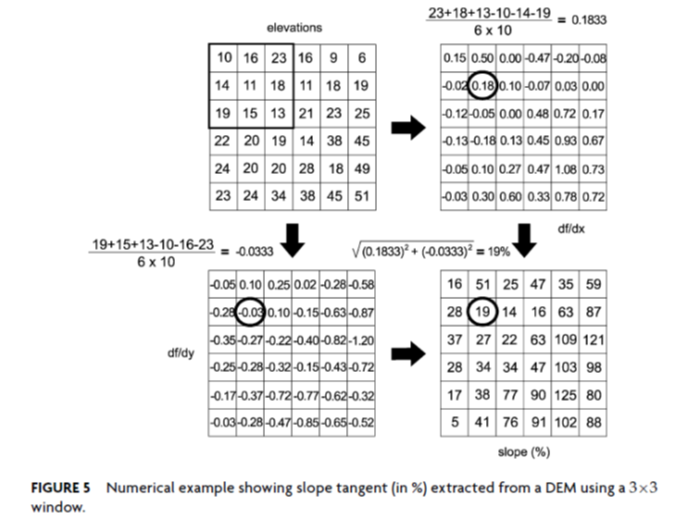
\includegraphics[height=.9\textheight]{pend}
    %\caption{This is the caption.}
  \end{figure}
\end{frame}
%################################SLIDE
\begin{frame}
\frametitle{Curvatura}
  \begin{figure}
    \centering
    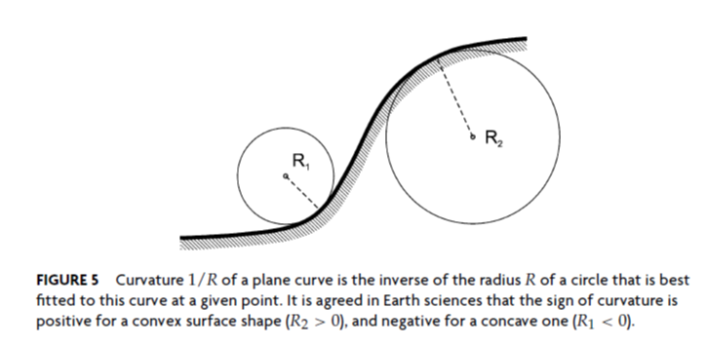
\includegraphics[height=.7\textheight]{curv}
    %\caption{This is the caption.}
  \end{figure}
\end{frame}
%################################SLIDE
\begin{frame}
%\framesubtitle{}
\begin{columns}
		\begin{column}{.50\linewidth}
		 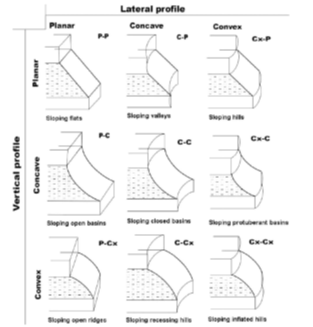
\includegraphics[width=6cm]{curv1}
		\end{column}
		\begin{column}{.50\linewidth}
			 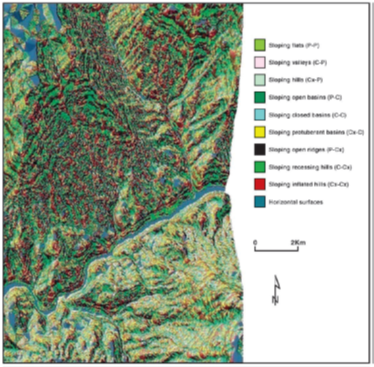
\includegraphics[width=6cm]{curv2}
		\end{column}
	\end{columns}
\end{frame}
%################################SLIDE
\begin{frame}
\frametitle{Perfiles}
  \begin{figure}
    \centering
    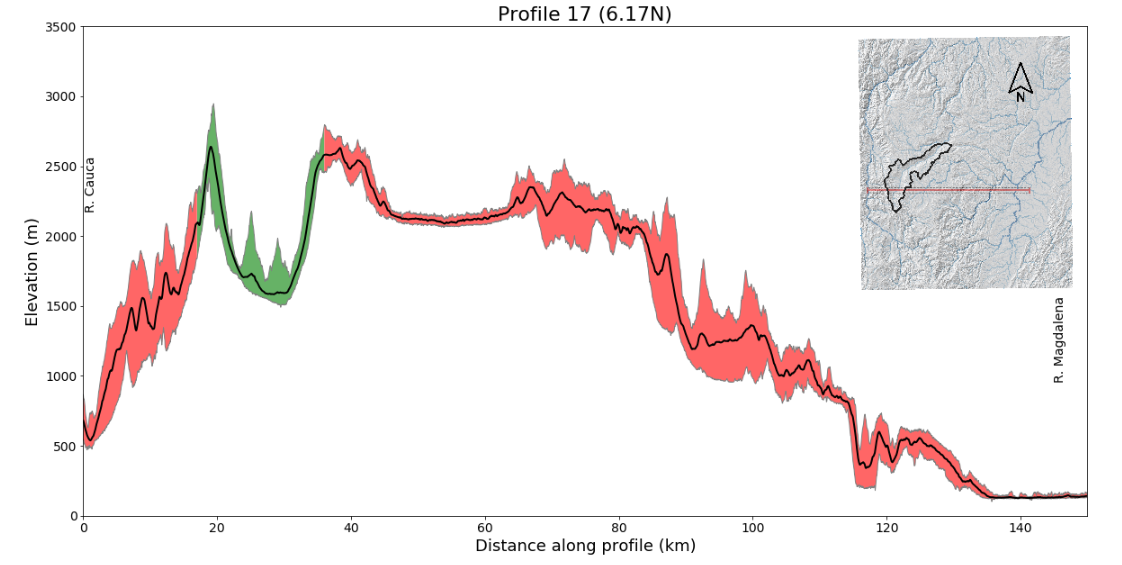
\includegraphics[height=.7\textheight]{profile}
    %\caption{This is the caption.}
  \end{figure}
\end{frame}
%################################SLIDE
\begin{frame}
\frametitle{Indices morfométricos}
  \begin{figure}
    \centering
    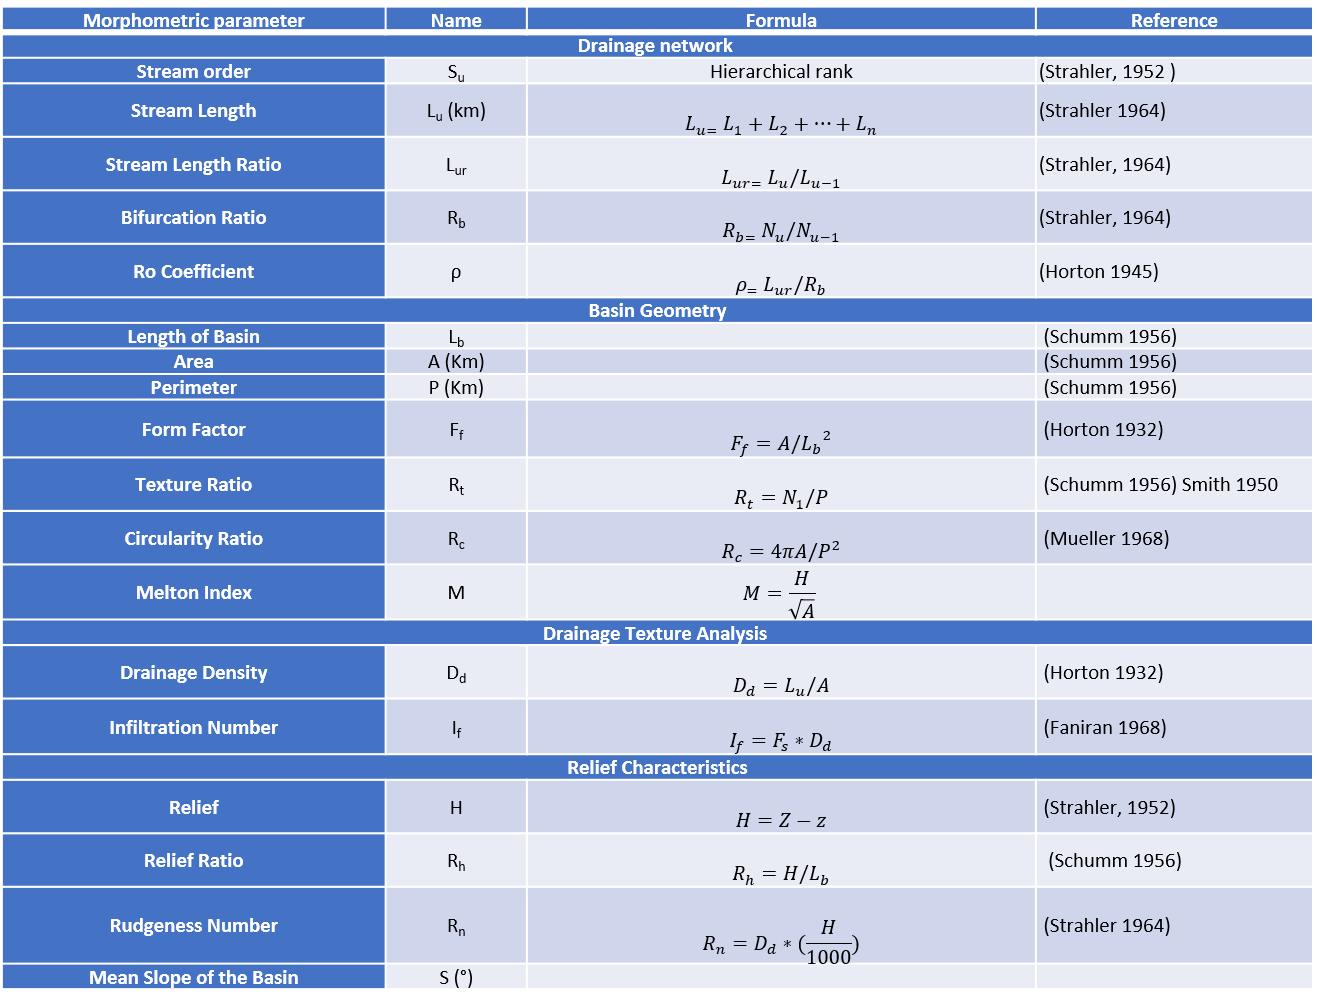
\includegraphics[height=.8\textheight]{indicestabla}
    %\caption{This is the caption.}
  \end{figure}
\end{frame}
%################################SLIDE
\begin{frame}
  \begin{figure}
    \centering
    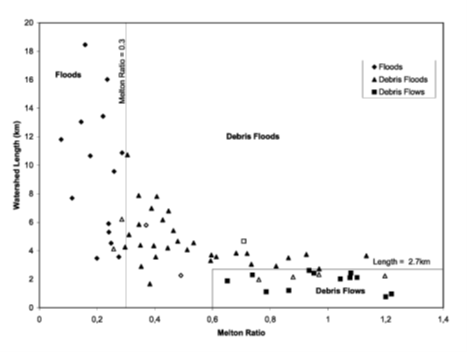
\includegraphics[height=.8\textheight]{melton}
    %\caption{This is the caption.}
  \end{figure}
\tiny{Fuente: Wilford et al. (2004)}
\end{frame}
%################################SLIDE
\begin{frame}
\frametitle{Perfiles longitudinales}
  \begin{figure}
    \centering
    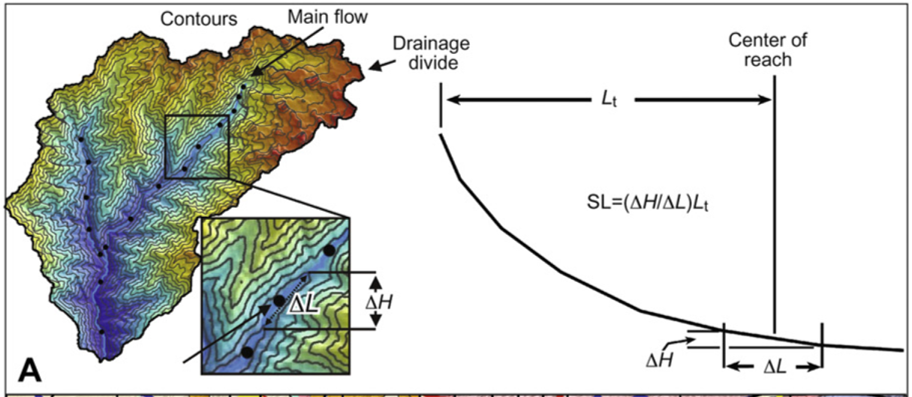
\includegraphics[height=.6\textheight]{long}
    %\caption{This is the caption.}
  \end{figure}
\tiny{}
\end{frame}
%################################SLIDE
\begin{frame}
  \begin{figure}
    \centering
    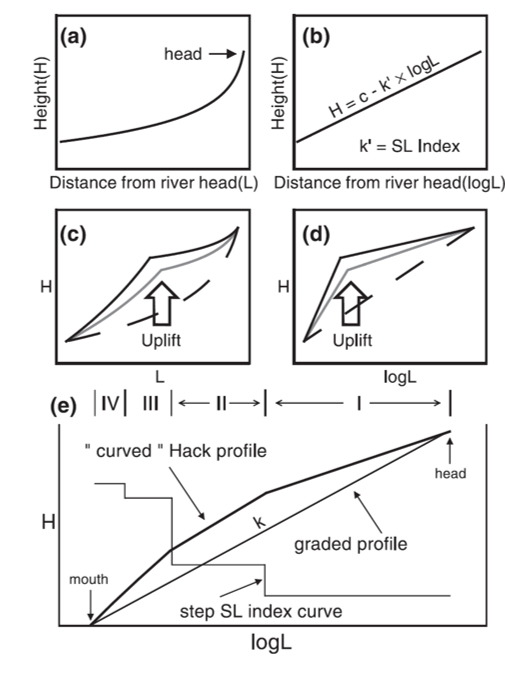
\includegraphics[height=.7\textheight]{hack}
    %\caption{This is the caption.}
  \end{figure}
\tiny{}
\end{frame}
%################################SLIDE
\begin{frame}
\frametitle{Curva hipsométrica}
  \begin{figure}
    \centering
    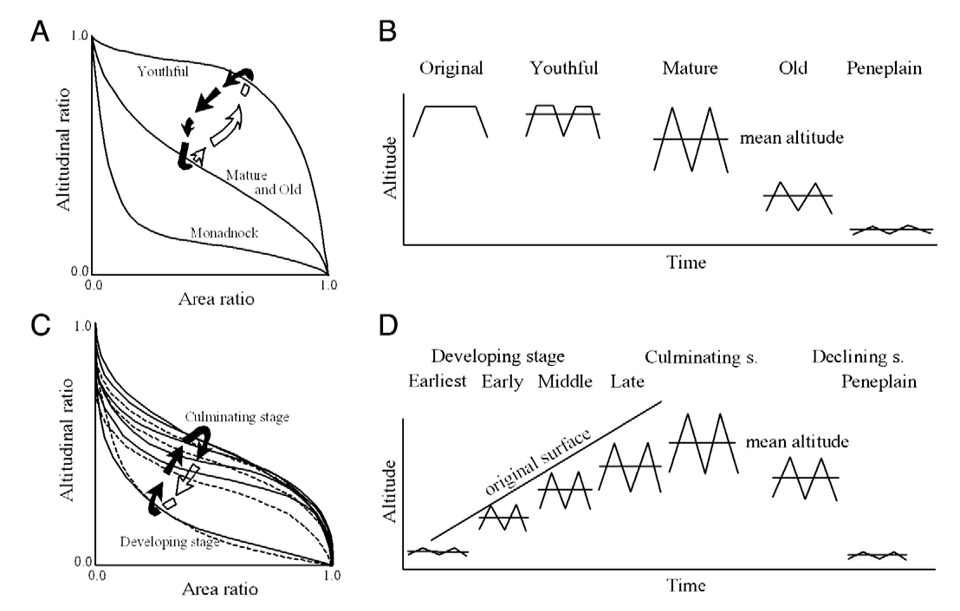
\includegraphics[height=.82\textheight]{hipsom}
    %\caption{This is the caption.}
  \end{figure}
\tiny{}
\end{frame}
%################################SLIDE
\begin{frame}
\frametitle{Indices tectónicos}
  \begin{figure}
    \centering
    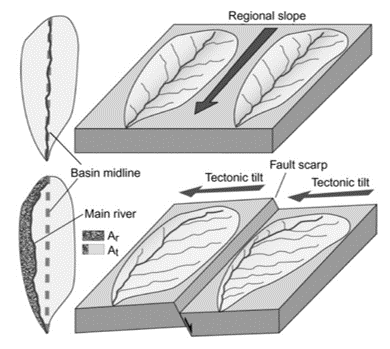
\includegraphics[height=.8\textheight]{tect}
    %\caption{This is the caption.}
  \end{figure}
\tiny{}
\end{frame}
%################################SLIDE
\begin{frame}
  \begin{figure}
    \centering
    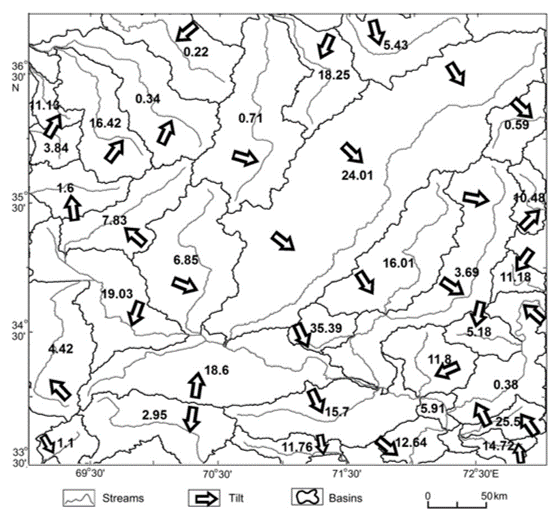
\includegraphics[height=.8\textheight]{tect2}
    %\caption{This is the caption.}
  \end{figure}
\tiny{}
\end{frame}
%################################SLIDE
\begin{frame}
\frametitle{Geomorfometría \& Análisis Hidrológico}
  \begin{figure}
    \centering
    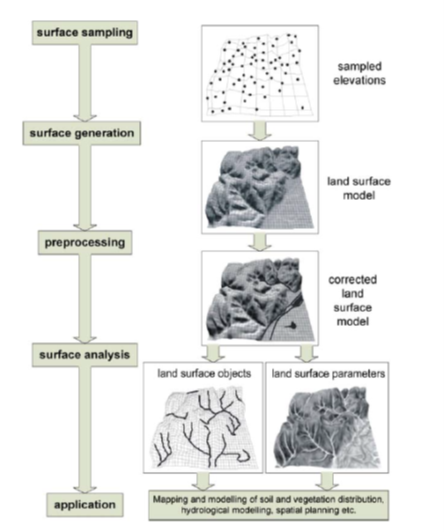
\includegraphics[height=.8\textheight]{hidro}
    %\caption{This is the caption.}
  \end{figure}
\end{frame}
%##############################SLIDE###########################################

\end{document}